\documentclass[1p]{elsarticle_modified}
%\bibliographystyle{elsarticle-num}

%\usepackage[colorlinks]{hyperref}
%\usepackage{abbrmath_seonhwa} %\Abb, \Ascr, \Acal ,\Abf, \Afrak
\usepackage{amsfonts}
\usepackage{amssymb}
\usepackage{amsmath}
\usepackage{amsthm}
\usepackage{scalefnt}
\usepackage{amsbsy}
\usepackage{kotex}
\usepackage{caption}
\usepackage{subfig}
\usepackage{color}
\usepackage{graphicx}
\usepackage{xcolor} %% white, black, red, green, blue, cyan, magenta, yellow
\usepackage{float}
\usepackage{setspace}
\usepackage{hyperref}

\usepackage{tikz}
\usetikzlibrary{arrows}

\usepackage{multirow}
\usepackage{array} % fixed length table
\usepackage{hhline}

%%%%%%%%%%%%%%%%%%%%%
\makeatletter
\renewcommand*\env@matrix[1][\arraystretch]{%
	\edef\arraystretch{#1}%
	\hskip -\arraycolsep
	\let\@ifnextchar\new@ifnextchar
	\array{*\c@MaxMatrixCols c}}
\makeatother %https://tex.stackexchange.com/questions/14071/how-can-i-increase-the-line-spacing-in-a-matrix
%%%%%%%%%%%%%%%

\usepackage[normalem]{ulem}

\newcommand{\msout}[1]{\ifmmode\text{\sout{\ensuremath{#1}}}\else\sout{#1}\fi}
%SOURCE: \msout is \stkout macro in https://tex.stackexchange.com/questions/20609/strikeout-in-math-mode

\newcommand{\cancel}[1]{
	\ifmmode
	{\color{red}\msout{#1}}
	\else
	{\color{red}\sout{#1}}
	\fi
}

\newcommand{\add}[1]{
	{\color{blue}\uwave{#1}}
}

\newcommand{\replace}[2]{
	\ifmmode
	{\color{red}\msout{#1}}{\color{blue}\uwave{#2}}
	\else
	{\color{red}\sout{#1}}{\color{blue}\uwave{#2}}
	\fi
}

\newcommand{\Sol}{\mathcal{S}} %segment
\newcommand{\D}{D} %diagram
\newcommand{\A}{\mathcal{A}} %arc


%%%%%%%%%%%%%%%%%%%%%%%%%%%%%5 test

\def\sl{\operatorname{\textup{SL}}(2,\Cbb)}
\def\psl{\operatorname{\textup{PSL}}(2,\Cbb)}
\def\quan{\mkern 1mu \triangleright \mkern 1mu}

\theoremstyle{definition}
\newtheorem{thm}{Theorem}[section]
\newtheorem{prop}[thm]{Proposition}
\newtheorem{lem}[thm]{Lemma}
\newtheorem{ques}[thm]{Question}
\newtheorem{cor}[thm]{Corollary}
\newtheorem{defn}[thm]{Definition}
\newtheorem{exam}[thm]{Example}
\newtheorem{rmk}[thm]{Remark}
\newtheorem{alg}[thm]{Algorithm}

\newcommand{\I}{\sqrt{-1}}
\begin{document}

%\begin{frontmatter}
%
%\title{Boundary parabolic representations of knots up to 8 crossings}
%
%%% Group authors per affiliation:
%\author{Yunhi Cho} 
%\address{Department of Mathematics, University of Seoul, Seoul, Korea}
%\ead{yhcho@uos.ac.kr}
%
%
%\author{Seonhwa Kim} %\fnref{s_kim}}
%\address{Center for Geometry and Physics, Institute for Basic Science, Pohang, 37673, Korea}
%\ead{ryeona17@ibs.re.kr}
%
%\author{Hyuk Kim}
%\address{Department of Mathematical Sciences, Seoul National University, Seoul 08826, Korea}
%\ead{hyukkim@snu.ac.kr}
%
%\author{Seokbeom Yoon}
%\address{Department of Mathematical Sciences, Seoul National University, Seoul, 08826,  Korea}
%\ead{sbyoon15@snu.ac.kr}
%
%\begin{abstract}
%We find all boundary parabolic representation of knots up to 8 crossings.
%
%\end{abstract}
%\begin{keyword}
%    \MSC[2010] 57M25 
%\end{keyword}
%
%\end{frontmatter}

%\linenumbers
%\tableofcontents
%
\newcommand\colored[1]{\textcolor{white}{\rule[-0.35ex]{0.8em}{1.4ex}}\kern-0.8em\color{red} #1}%
%\newcommand\colored[1]{\textcolor{white}{ #1}\kern-2.17ex	\textcolor{white}{ #1}\kern-1.81ex	\textcolor{white}{ #1}\kern-2.15ex\color{red}#1	}

{\Large $\underline{12n_{0820}~(K12n_{0820})}$}

\setlength{\tabcolsep}{10pt}
\renewcommand{\arraystretch}{1.6}
\vspace{1cm}\begin{tabular}{m{100pt}>{\centering\arraybackslash}m{274pt}}
\multirow{5}{120pt}{
	\centering
	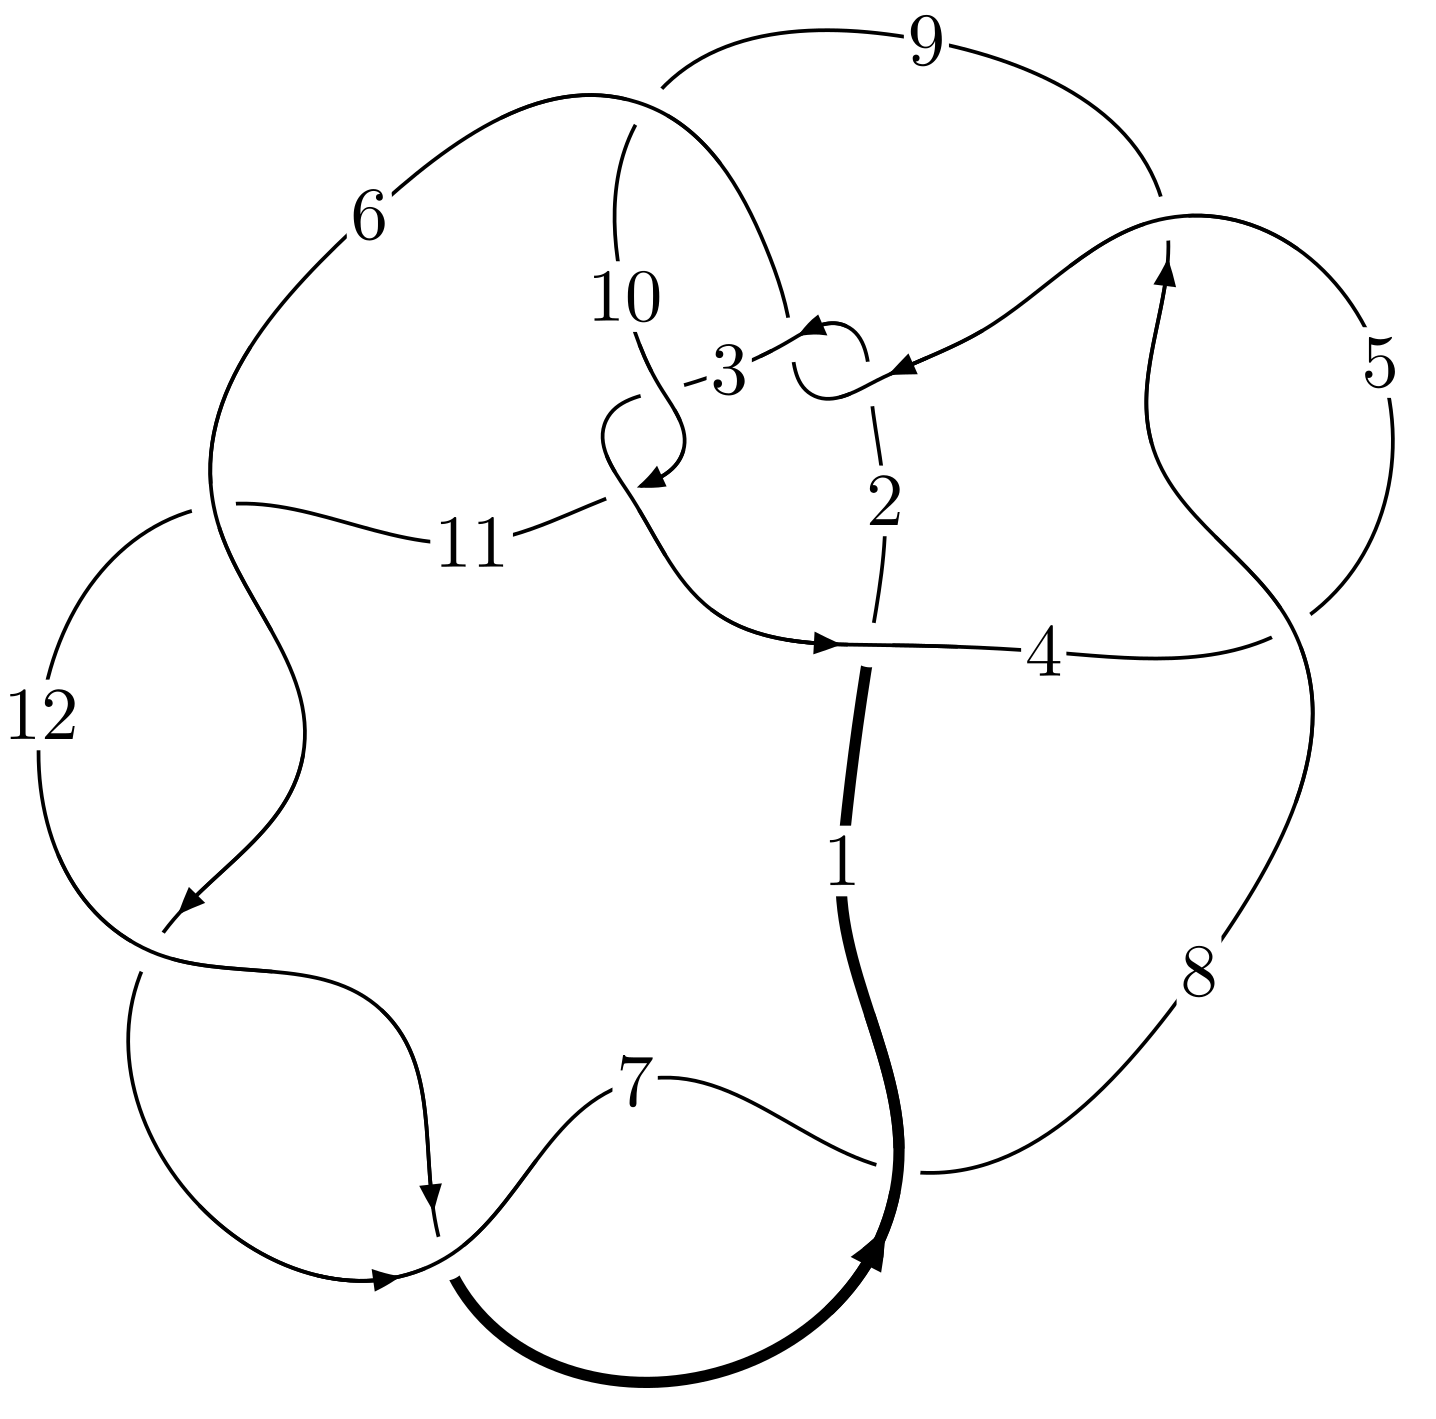
\includegraphics[width=112pt]{../../../GIT/diagram.site/Diagrams/png/2909_12n_0820.png}\\
\ \ \ A knot diagram\footnotemark}&
\allowdisplaybreaks
\textbf{Linearized knot diagam} \\
\cline{2-2}
 &
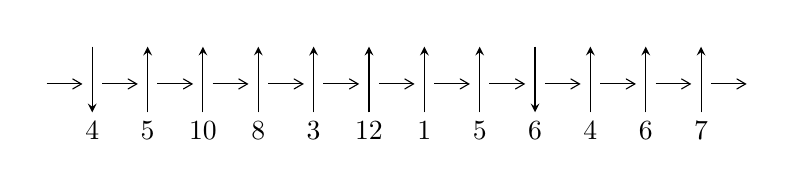
\begin{tikzpicture}[x=20pt, y=17pt]
	% nodes
	\node (C0) at (0, 0) {};
	\node (C1) at (1, 0) {};
	\node (C1U) at (1, +1) {};
	\node (C1D) at (1, -1) {4};

	\node (C2) at (2, 0) {};
	\node (C2U) at (2, +1) {};
	\node (C2D) at (2, -1) {5};

	\node (C3) at (3, 0) {};
	\node (C3U) at (3, +1) {};
	\node (C3D) at (3, -1) {10};

	\node (C4) at (4, 0) {};
	\node (C4U) at (4, +1) {};
	\node (C4D) at (4, -1) {8};

	\node (C5) at (5, 0) {};
	\node (C5U) at (5, +1) {};
	\node (C5D) at (5, -1) {3};

	\node (C6) at (6, 0) {};
	\node (C6U) at (6, +1) {};
	\node (C6D) at (6, -1) {12};

	\node (C7) at (7, 0) {};
	\node (C7U) at (7, +1) {};
	\node (C7D) at (7, -1) {1};

	\node (C8) at (8, 0) {};
	\node (C8U) at (8, +1) {};
	\node (C8D) at (8, -1) {5};

	\node (C9) at (9, 0) {};
	\node (C9U) at (9, +1) {};
	\node (C9D) at (9, -1) {6};

	\node (C10) at (10, 0) {};
	\node (C10U) at (10, +1) {};
	\node (C10D) at (10, -1) {4};

	\node (C11) at (11, 0) {};
	\node (C11U) at (11, +1) {};
	\node (C11D) at (11, -1) {6};

	\node (C12) at (12, 0) {};
	\node (C12U) at (12, +1) {};
	\node (C12D) at (12, -1) {7};
	\node (C13) at (13, 0) {};

	% arrows
	\draw[->,>={angle 60}]
	(C0) edge (C1) (C1) edge (C2) (C2) edge (C3) (C3) edge (C4) (C4) edge (C5) (C5) edge (C6) (C6) edge (C7) (C7) edge (C8) (C8) edge (C9) (C9) edge (C10) (C10) edge (C11) (C11) edge (C12) (C12) edge (C13) ;	\draw[->,>=stealth]
	(C1U) edge (C1D) (C2D) edge (C2U) (C3D) edge (C3U) (C4D) edge (C4U) (C5D) edge (C5U) (C6D) edge (C6U) (C7D) edge (C7U) (C8D) edge (C8U) (C9U) edge (C9D) (C10D) edge (C10U) (C11D) edge (C11U) (C12D) edge (C12U) ;
	\end{tikzpicture} \\
\hhline{~~} \\& 
\textbf{Solving Sequence} \\ \cline{2-2} 
 &
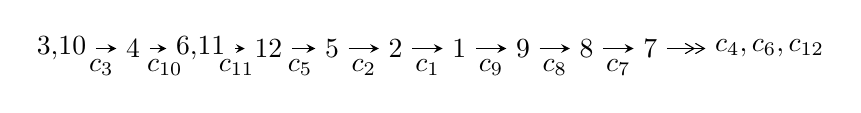
\begin{tikzpicture}[x=23pt, y=7pt]
	% node
	\node (A0) at (-1/8, 0) {3,10};
	\node (A1) at (1, 0) {4};
	\node (A2) at (33/16, 0) {6,11};
	\node (A3) at (25/8, 0) {12};
	\node (A4) at (33/8, 0) {5};
	\node (A5) at (41/8, 0) {2};
	\node (A6) at (49/8, 0) {1};
	\node (A7) at (57/8, 0) {9};
	\node (A8) at (65/8, 0) {8};
	\node (A9) at (73/8, 0) {7};
	\node (C1) at (1/2, -1) {$c_{3}$};
	\node (C2) at (3/2, -1) {$c_{10}$};
	\node (C3) at (21/8, -1) {$c_{11}$};
	\node (C4) at (29/8, -1) {$c_{5}$};
	\node (C5) at (37/8, -1) {$c_{2}$};
	\node (C6) at (45/8, -1) {$c_{1}$};
	\node (C7) at (53/8, -1) {$c_{9}$};
	\node (C8) at (61/8, -1) {$c_{8}$};
	\node (C9) at (69/8, -1) {$c_{7}$};
	\node (A10) at (11, 0) {$c_{4},c_{6},c_{12}$};

	% edge
	\draw[->,>=stealth]	
	(A0) edge (A1) (A1) edge (A2) (A2) edge (A3) (A3) edge (A4) (A4) edge (A5) (A5) edge (A6) (A6) edge (A7) (A7) edge (A8) (A8) edge (A9) ;
	\draw[->>,>={angle 60}]	
	(A9) edge (A10);
\end{tikzpicture} \\ 

\end{tabular} \\

\footnotetext{
The image of knot diagram is generated by the software ``\textbf{Draw programme}" developed by Andrew Bartholomew(\url{http://www.layer8.co.uk/maths/draw/index.htm\#Running-draw}), where we modified some parts for our purpose(\url{https://github.com/CATsTAILs/LinksPainter}).
}\phantom \\ \newline 
\centering \textbf{Ideals for irreducible components\footnotemark of $X_{\text{par}}$} 
 
\begin{align*}
I^u_{1}&=\langle 
20309 u^{19}+9314 u^{18}+\cdots+12371 b-15594,\;980 u^{19}+5579 u^{18}+\cdots+12371 a-1467,\\
\phantom{I^u_{1}}&\phantom{= \langle  }u^{20}+u^{19}+\cdots-2 u-1\rangle \\
I^u_{2}&=\langle 
7.00656\times10^{35} u^{35}+1.59035\times10^{36} u^{34}+\cdots+1.29954\times10^{37} b-3.85421\times10^{38},\\
\phantom{I^u_{2}}&\phantom{= \langle  }1.69263\times10^{47} u^{35}-2.24834\times10^{47} u^{34}+\cdots+5.15433\times10^{47} a+1.11901\times10^{49},\;u^{36}- u^{35}+\cdots-50 u+173\rangle \\
I^u_{3}&=\langle 
u^{10}+u^9-4 u^8-4 u^7+4 u^6+5 u^5-2 u^4-3 u^3+2 u^2+b+u+1,\\
\phantom{I^u_{3}}&\phantom{= \langle  }u^{10}-6 u^8+13 u^6+u^5-15 u^4-2 u^3+12 u^2+a-4,\\
\phantom{I^u_{3}}&\phantom{= \langle  }u^{11}+u^{10}-5 u^9-5 u^8+8 u^7+9 u^6-6 u^5-8 u^4+4 u^3+4 u^2- u-1\rangle \\
\\
\end{align*}
\raggedright * 3 irreducible components of $\dim_{\mathbb{C}}=0$, with total 67 representations.\\
\footnotetext{All coefficients of polynomials are rational numbers. But the coefficients are sometimes approximated in decimal forms when there is not enough margin.}
\newpage
\renewcommand{\arraystretch}{1}
\centering \section*{I. $I^u_{1}= \langle 20309 u^{19}+9314 u^{18}+\cdots+12371 b-15594,\;980 u^{19}+5579 u^{18}+\cdots+12371 a-1467,\;u^{20}+u^{19}+\cdots-2 u-1 \rangle$}
\flushleft \textbf{(i) Arc colorings}\\
\begin{tabular}{m{7pt} m{180pt} m{7pt} m{180pt} }
\flushright $a_{3}=$&$\begin{pmatrix}1\\0\end{pmatrix}$ \\
\flushright $a_{10}=$&$\begin{pmatrix}0\\u\end{pmatrix}$ \\
\flushright $a_{4}=$&$\begin{pmatrix}1\\- u^2\end{pmatrix}$ \\
\flushright $a_{6}=$&$\begin{pmatrix}-0.0792175 u^{19}-0.450974 u^{18}+\cdots-1.69647 u+0.118584\\-1.64166 u^{19}-0.752890 u^{18}+\cdots+0.958613 u+1.26053\end{pmatrix}$ \\
\flushright $a_{11}=$&$\begin{pmatrix}u\\- u^3+u\end{pmatrix}$ \\
\flushright $a_{12}=$&$\begin{pmatrix}0.881416 u^{19}+0.960634 u^{18}+\cdots+2.54110 u-0.0663649\\1.12651 u^{19}+0.184464 u^{18}+\cdots-2.07146 u-2.24549\end{pmatrix}$ \\
\flushright $a_{5}=$&$\begin{pmatrix}1.56244 u^{19}+0.301916 u^{18}+\cdots-2.65508 u-1.14194\\-1.64166 u^{19}-0.752890 u^{18}+\cdots+0.958613 u+1.26053\end{pmatrix}$ \\
\flushright $a_{2}=$&$\begin{pmatrix}-2.04009 u^{19}-0.999677 u^{18}+\cdots-1.51984 u+2.04777\\1.96088 u^{19}+0.548703 u^{18}+\cdots-0.176623 u-1.92919\end{pmatrix}$ \\
\flushright $a_{1}=$&$\begin{pmatrix}-0.603832 u^{19}-0.366098 u^{18}+\cdots-1.65573 u+1.15900\\0.942042 u^{19}+0.234338 u^{18}+\cdots-0.00751758 u-1.12651\end{pmatrix}$ \\
\flushright $a_{9}=$&$\begin{pmatrix}0.881416 u^{19}+0.960634 u^{18}+\cdots+1.54110 u-0.0663649\\-0.371757 u^{19}-0.166357 u^{18}+\cdots-0.0398513 u-0.0792175\end{pmatrix}$ \\
\flushright $a_{8}=$&$\begin{pmatrix}2.14194 u^{19}+0.579500 u^{18}+\cdots-0.441840 u-1.62881\\-1.26053 u^{19}+0.381133 u^{18}+\cdots+1.98294 u+1.56244\end{pmatrix}$ \\
\flushright $a_{7}=$&$\begin{pmatrix}-2.36408 u^{19}-0.158354 u^{18}+\cdots+1.84399 u+3.35316\\3.06855 u^{19}+0.418802 u^{18}+\cdots-3.07898 u-4.37200\end{pmatrix}$\\&\end{tabular}
\flushleft \textbf{(ii) Obstruction class $= -1$}\\~\\
\flushleft \textbf{(iii) Cusp Shapes $= \frac{108774}{12371} u^{19}+\frac{59182}{12371} u^{18}+\cdots+\frac{1686}{12371} u+\frac{115368}{12371}$}\\~\\
\newpage\renewcommand{\arraystretch}{1}
\flushleft \textbf{(iv) u-Polynomials at the component}\newline \\
\begin{tabular}{m{50pt}|m{274pt}}
Crossings & \hspace{64pt}u-Polynomials at each crossing \\
\hline $$\begin{aligned}c_{1}\end{aligned}$$&$\begin{aligned}
&u^{20}- u^{19}+\cdots+3 u-1
\end{aligned}$\\
\hline $$\begin{aligned}c_{2},c_{5}\end{aligned}$$&$\begin{aligned}
&u^{20}+12 u^{19}+\cdots-288 u-64
\end{aligned}$\\
\hline $$\begin{aligned}c_{3},c_{4},c_{8}\\c_{10}\end{aligned}$$&$\begin{aligned}
&u^{20}- u^{19}+\cdots+2 u-1
\end{aligned}$\\
\hline $$\begin{aligned}c_{6},c_{7},c_{11}\\c_{12}\end{aligned}$$&$\begin{aligned}
&u^{20}-7 u^{19}+\cdots-16 u+8
\end{aligned}$\\
\hline $$\begin{aligned}c_{9}\end{aligned}$$&$\begin{aligned}
&u^{20}-7 u^{18}+\cdots-3 u+1
\end{aligned}$\\
\hline
\end{tabular}\\~\\
\newpage\renewcommand{\arraystretch}{1}
\flushleft \textbf{(v) Riley Polynomials at the component}\newline \\
\begin{tabular}{m{50pt}|m{274pt}}
Crossings & \hspace{64pt}Riley Polynomials at each crossing \\
\hline $$\begin{aligned}c_{1}\end{aligned}$$&$\begin{aligned}
&y^{20}-9 y^{19}+\cdots-23 y+1
\end{aligned}$\\
\hline $$\begin{aligned}c_{2},c_{5}\end{aligned}$$&$\begin{aligned}
&y^{20}-12 y^{19}+\cdots-41984 y+4096
\end{aligned}$\\
\hline $$\begin{aligned}c_{3},c_{4},c_{8}\\c_{10}\end{aligned}$$&$\begin{aligned}
&y^{20}-7 y^{19}+\cdots-12 y+1
\end{aligned}$\\
\hline $$\begin{aligned}c_{6},c_{7},c_{11}\\c_{12}\end{aligned}$$&$\begin{aligned}
&y^{20}-23 y^{19}+\cdots-480 y+64
\end{aligned}$\\
\hline $$\begin{aligned}c_{9}\end{aligned}$$&$\begin{aligned}
&y^{20}-14 y^{19}+\cdots-47 y+1
\end{aligned}$\\
\hline
\end{tabular}\\~\\
\newpage\flushleft \textbf{(vi) Complex Volumes and Cusp Shapes}
$$\begin{array}{c|c|c}  
\text{Solutions to }I^u_{1}& \I (\text{vol} + \sqrt{-1}CS) & \text{Cusp shape}\\
 \hline 
\begin{aligned}
u &= \phantom{-}0.531641 + 0.775820 I \\
a &= \phantom{-}0.521652 - 0.793900 I \\
b &= \phantom{-}0.421927 - 0.879767 I\end{aligned}
 & -2.87838 + 0.48775 I & \phantom{-}4.90275 - 0.25050 I \\ \hline\begin{aligned}
u &= \phantom{-}0.531641 - 0.775820 I \\
a &= \phantom{-}0.521652 + 0.793900 I \\
b &= \phantom{-}0.421927 + 0.879767 I\end{aligned}
 & -2.87838 - 0.48775 I & \phantom{-}4.90275 + 0.25050 I \\ \hline\begin{aligned}
u &= -0.780003 + 0.720862 I \\
a &= \phantom{-}0.368240 + 0.692494 I \\
b &= \phantom{-}0.401381 + 1.125740 I\end{aligned}
 & -1.50723 - 4.46688 I & \phantom{-}9.00256 + 6.89614 I \\ \hline\begin{aligned}
u &= -0.780003 - 0.720862 I \\
a &= \phantom{-}0.368240 - 0.692494 I \\
b &= \phantom{-}0.401381 - 1.125740 I\end{aligned}
 & -1.50723 + 4.46688 I & \phantom{-}9.00256 - 6.89614 I \\ \hline\begin{aligned}
u &= -0.918199\phantom{ +0.000000I} \\
a &= -1.32642\phantom{ +0.000000I} \\
b &= \phantom{-}1.75391\phantom{ +0.000000I}\end{aligned}
 & \phantom{-}16.1040\phantom{ +0.000000I} & \phantom{-}18.7100\phantom{ +0.000000I} \\ \hline\begin{aligned}
u &= -0.173666 + 0.881491 I \\
a &= \phantom{-}0.646323 + 1.135580 I \\
b &= \phantom{-}0.621428 + 0.665143 I\end{aligned}
 & \phantom{-}2.15657 + 2.07163 I & \phantom{-}8.70820 - 2.09392 I \\ \hline\begin{aligned}
u &= -0.173666 - 0.881491 I \\
a &= \phantom{-}0.646323 - 1.135580 I \\
b &= \phantom{-}0.621428 - 0.665143 I\end{aligned}
 & \phantom{-}2.15657 - 2.07163 I & \phantom{-}8.70820 + 2.09392 I \\ \hline\begin{aligned}
u &= \phantom{-}0.773890 + 0.398773 I \\
a &= -1.14329 + 1.51420 I \\
b &= \phantom{-}1.317590 + 0.420622 I\end{aligned}
 & \phantom{-}4.34968 + 1.79622 I & \phantom{-}15.4727 - 7.2361 I \\ \hline\begin{aligned}
u &= \phantom{-}0.773890 - 0.398773 I \\
a &= -1.14329 - 1.51420 I \\
b &= \phantom{-}1.317590 - 0.420622 I\end{aligned}
 & \phantom{-}4.34968 - 1.79622 I & \phantom{-}15.4727 + 7.2361 I \\ \hline\begin{aligned}
u &= -0.964251 + 0.670604 I \\
a &= -0.50985 - 1.33705 I \\
b &= \phantom{-}1.248990 - 0.652969 I\end{aligned}
 & -0.28761 - 6.25899 I & \phantom{-}10.23267 + 5.61351 I\\
 \hline 
 \end{array}$$\newpage$$\begin{array}{c|c|c}  
\text{Solutions to }I^u_{1}& \I (\text{vol} + \sqrt{-1}CS) & \text{Cusp shape}\\
 \hline 
\begin{aligned}
u &= -0.964251 - 0.670604 I \\
a &= -0.50985 + 1.33705 I \\
b &= \phantom{-}1.248990 + 0.652969 I\end{aligned}
 & -0.28761 + 6.25899 I & \phantom{-}10.23267 - 5.61351 I \\ \hline\begin{aligned}
u &= \phantom{-}0.971344 + 0.669842 I \\
a &= \phantom{-}0.253502 - 0.657470 I \\
b &= \phantom{-}0.489453 - 1.324130 I\end{aligned}
 & \phantom{-}6.46708 + 7.19476 I & \phantom{-}12.8367 - 6.4139 I \\ \hline\begin{aligned}
u &= \phantom{-}0.971344 - 0.669842 I \\
a &= \phantom{-}0.253502 + 0.657470 I \\
b &= \phantom{-}0.489453 + 1.324130 I\end{aligned}
 & \phantom{-}6.46708 - 7.19476 I & \phantom{-}12.8367 + 6.4139 I \\ \hline\begin{aligned}
u &= -0.783799\phantom{ +0.000000I} \\
a &= \phantom{-}0.321973\phantom{ +0.000000I} \\
b &= -2.10585\phantom{ +0.000000I}\end{aligned}
 & \phantom{-}15.5209\phantom{ +0.000000I} & \phantom{-}28.3760\phantom{ +0.000000I} \\ \hline\begin{aligned}
u &= \phantom{-}0.696724\phantom{ +0.000000I} \\
a &= \phantom{-}0.426342\phantom{ +0.000000I} \\
b &= -1.34554\phantom{ +0.000000I}\end{aligned}
 & \phantom{-}5.26045\phantom{ +0.000000I} & \phantom{-}19.7990\phantom{ +0.000000I} \\ \hline\begin{aligned}
u &= \phantom{-}1.163650 + 0.737004 I \\
a &= -0.392518 + 1.185430 I \\
b &= \phantom{-}1.25173 + 0.76023 I\end{aligned}
 & \phantom{-}1.08242 + 11.20720 I & \phantom{-}12.2004 - 8.8347 I \\ \hline\begin{aligned}
u &= \phantom{-}1.163650 - 0.737004 I \\
a &= -0.392518 - 1.185430 I \\
b &= \phantom{-}1.25173 - 0.76023 I\end{aligned}
 & \phantom{-}1.08242 - 11.20720 I & \phantom{-}12.2004 + 8.8347 I \\ \hline\begin{aligned}
u &= -1.32603 + 0.74385 I \\
a &= -0.336093 - 1.104220 I \\
b &= \phantom{-}1.25227 - 0.82883 I\end{aligned}
 & \phantom{-}8.8703 - 14.6138 I & \phantom{-}14.9115 + 7.7101 I \\ \hline\begin{aligned}
u &= -1.32603 - 0.74385 I \\
a &= -0.336093 + 1.104220 I \\
b &= \phantom{-}1.25227 + 0.82883 I\end{aligned}
 & \phantom{-}8.8703 + 14.6138 I & \phantom{-}14.9115 - 7.7101 I \\ \hline\begin{aligned}
u &= -0.387870\phantom{ +0.000000I} \\
a &= \phantom{-}0.762165\phantom{ +0.000000I} \\
b &= -0.312052\phantom{ +0.000000I}\end{aligned}
 & \phantom{-}0.631092\phantom{ +0.000000I} & \phantom{-}15.5800\phantom{ +0.000000I}\\
 \hline 
 \end{array}$$\newpage\newpage\renewcommand{\arraystretch}{1}
\centering \section*{II. $I^u_{2}= \langle 7.01\times10^{35} u^{35}+1.59\times10^{36} u^{34}+\cdots+1.30\times10^{37} b-3.85\times10^{38},\;1.69\times10^{47} u^{35}-2.25\times10^{47} u^{34}+\cdots+5.15\times10^{47} a+1.12\times10^{49},\;u^{36}- u^{35}+\cdots-50 u+173 \rangle$}
\flushleft \textbf{(i) Arc colorings}\\
\begin{tabular}{m{7pt} m{180pt} m{7pt} m{180pt} }
\flushright $a_{3}=$&$\begin{pmatrix}1\\0\end{pmatrix}$ \\
\flushright $a_{10}=$&$\begin{pmatrix}0\\u\end{pmatrix}$ \\
\flushright $a_{4}=$&$\begin{pmatrix}1\\- u^2\end{pmatrix}$ \\
\flushright $a_{6}=$&$\begin{pmatrix}-0.328391 u^{35}+0.436204 u^{34}+\cdots+113.808 u-21.7102\\-0.0539155 u^{35}-0.122378 u^{34}+\cdots+22.7256 u+29.6582\end{pmatrix}$ \\
\flushright $a_{11}=$&$\begin{pmatrix}u\\- u^3+u\end{pmatrix}$ \\
\flushright $a_{12}=$&$\begin{pmatrix}-0.00968600 u^{35}+0.0510508 u^{34}+\cdots+1.34871 u-1.93665\\0.00857854 u^{35}-0.0342699 u^{34}+\cdots-13.5525 u+19.8135\end{pmatrix}$ \\
\flushright $a_{5}=$&$\begin{pmatrix}-0.274475 u^{35}+0.558582 u^{34}+\cdots+91.0822 u-51.3684\\-0.0539155 u^{35}-0.122378 u^{34}+\cdots+22.7256 u+29.6582\end{pmatrix}$ \\
\flushright $a_{2}=$&$\begin{pmatrix}-0.0588044 u^{35}+0.0152006 u^{34}+\cdots+28.6506 u+1.10313\\0.136673 u^{35}-0.144683 u^{34}+\cdots-51.6170 u+2.13006\end{pmatrix}$ \\
\flushright $a_{1}=$&$\begin{pmatrix}0.0979711 u^{35}-0.205251 u^{34}+\cdots-14.9735 u+10.7766\\0.0485802 u^{35}-0.0205206 u^{34}+\cdots-21.3111 u-8.88587\end{pmatrix}$ \\
\flushright $a_{9}=$&$\begin{pmatrix}-0.108106 u^{35}+0.223334 u^{34}+\cdots+30.9390 u-35.3423\\-0.0516142 u^{35}+0.107338 u^{34}+\cdots+7.12661 u-13.4712\end{pmatrix}$ \\
\flushright $a_{8}=$&$\begin{pmatrix}0.189528 u^{35}-0.272285 u^{34}+\cdots-33.3725 u+19.4151\\-0.163428 u^{35}+0.181105 u^{34}+\cdots+19.8997 u+14.8460\end{pmatrix}$ \\
\flushright $a_{7}=$&$\begin{pmatrix}0.420493 u^{35}-0.834327 u^{34}+\cdots-109.957 u+116.513\\-0.177158 u^{35}+0.159116 u^{34}+\cdots+31.9669 u+13.1878\end{pmatrix}$\\&\end{tabular}
\flushleft \textbf{(ii) Obstruction class $= -1$}\\~\\
\flushleft \textbf{(iii) Cusp Shapes $= -0.185352 u^{35}+0.112252 u^{34}+\cdots+117.655 u+30.4332$}\\~\\
\newpage\renewcommand{\arraystretch}{1}
\flushleft \textbf{(iv) u-Polynomials at the component}\newline \\
\begin{tabular}{m{50pt}|m{274pt}}
Crossings & \hspace{64pt}u-Polynomials at each crossing \\
\hline $$\begin{aligned}c_{1}\end{aligned}$$&$\begin{aligned}
&u^{36}-7 u^{35}+\cdots+556 u+23
\end{aligned}$\\
\hline $$\begin{aligned}c_{2},c_{5}\end{aligned}$$&$\begin{aligned}
&(u^3- u^2+1)^{12}
\end{aligned}$\\
\hline $$\begin{aligned}c_{3},c_{4},c_{8}\\c_{10}\end{aligned}$$&$\begin{aligned}
&u^{36}+u^{35}+\cdots+50 u+173
\end{aligned}$\\
\hline $$\begin{aligned}c_{6},c_{7},c_{11}\\c_{12}\end{aligned}$$&$\begin{aligned}
&(u^6+u^5-3 u^4-2 u^3+2 u^2- u-1)^6
\end{aligned}$\\
\hline $$\begin{aligned}c_{9}\end{aligned}$$&$\begin{aligned}
&u^{36}+3 u^{35}+\cdots-268 u-1
\end{aligned}$\\
\hline
\end{tabular}\\~\\
\newpage\renewcommand{\arraystretch}{1}
\flushleft \textbf{(v) Riley Polynomials at the component}\newline \\
\begin{tabular}{m{50pt}|m{274pt}}
Crossings & \hspace{64pt}Riley Polynomials at each crossing \\
\hline $$\begin{aligned}c_{1}\end{aligned}$$&$\begin{aligned}
&y^{36}+15 y^{35}+\cdots-395064 y+529
\end{aligned}$\\
\hline $$\begin{aligned}c_{2},c_{5}\end{aligned}$$&$\begin{aligned}
&(y^3- y^2+2 y-1)^{12}
\end{aligned}$\\
\hline $$\begin{aligned}c_{3},c_{4},c_{8}\\c_{10}\end{aligned}$$&$\begin{aligned}
&y^{36}-21 y^{35}+\cdots-421852 y+29929
\end{aligned}$\\
\hline $$\begin{aligned}c_{6},c_{7},c_{11}\\c_{12}\end{aligned}$$&$\begin{aligned}
&(y^6-7 y^5+17 y^4-16 y^3+6 y^2-5 y+1)^6
\end{aligned}$\\
\hline $$\begin{aligned}c_{9}\end{aligned}$$&$\begin{aligned}
&y^{36}+7 y^{35}+\cdots-70616 y+1
\end{aligned}$\\
\hline
\end{tabular}\\~\\
\newpage\flushleft \textbf{(vi) Complex Volumes and Cusp Shapes}
$$\begin{array}{c|c|c}  
\text{Solutions to }I^u_{2}& \I (\text{vol} + \sqrt{-1}CS) & \text{Cusp shape}\\
 \hline 
\begin{aligned}
u &= \phantom{-}0.680331 + 0.769624 I \\
a &= \phantom{-}0.857359 - 0.939810 I \\
b &= -0.877439 - 0.744862 I\end{aligned}
 & \phantom{-}5.60625 - 1.76400 I & \phantom{-}13.07138 + 0.22537 I \\ \hline\begin{aligned}
u &= \phantom{-}0.680331 - 0.769624 I \\
a &= \phantom{-}0.857359 + 0.939810 I \\
b &= -0.877439 + 0.744862 I\end{aligned}
 & \phantom{-}5.60625 + 1.76400 I & \phantom{-}13.07138 - 0.22537 I \\ \hline\begin{aligned}
u &= -0.715828 + 0.752424 I \\
a &= -0.440309 - 0.292593 I \\
b &= -0.877439 - 0.744862 I\end{aligned}
 & -1.049570 + 0.855710 I & \phantom{-}9.06597 + 0.70533 I \\ \hline\begin{aligned}
u &= -0.715828 - 0.752424 I \\
a &= -0.440309 + 0.292593 I \\
b &= -0.877439 + 0.744862 I\end{aligned}
 & -1.049570 - 0.855710 I & \phantom{-}9.06597 - 0.70533 I \\ \hline\begin{aligned}
u &= -0.808909 + 0.653470 I \\
a &= -0.279403 + 0.967994 I \\
b &= -0.877439 + 0.744862 I\end{aligned}
 & \phantom{-}2.64952 - 2.82812 I & \phantom{-}17.9070 + 2.9794 I \\ \hline\begin{aligned}
u &= -0.808909 - 0.653470 I \\
a &= -0.279403 - 0.967994 I \\
b &= -0.877439 - 0.744862 I\end{aligned}
 & \phantom{-}2.64952 + 2.82812 I & \phantom{-}17.9070 - 2.9794 I \\ \hline\begin{aligned}
u &= -0.902191 + 0.566521 I \\
a &= \phantom{-}0.392677 - 1.208180 I \\
b &= \phantom{-}0.754878\phantom{ +0.000000I}\end{aligned}
 & \phantom{-}3.08801 - 1.97241 I & \phantom{-}15.5952 + 3.6848 I \\ \hline\begin{aligned}
u &= -0.902191 - 0.566521 I \\
a &= \phantom{-}0.392677 + 1.208180 I \\
b &= \phantom{-}0.754878\phantom{ +0.000000I}\end{aligned}
 & \phantom{-}3.08801 + 1.97241 I & \phantom{-}15.5952 - 3.6848 I \\ \hline\begin{aligned}
u &= -0.907127 + 0.187470 I \\
a &= -1.51181 + 1.66928 I \\
b &= \phantom{-}0.754878\phantom{ +0.000000I}\end{aligned}
 & \phantom{-}9.74383 - 4.59213 I & \phantom{-}19.6006 + 3.2048 I \\ \hline\begin{aligned}
u &= -0.907127 - 0.187470 I \\
a &= -1.51181 - 1.66928 I \\
b &= \phantom{-}0.754878\phantom{ +0.000000I}\end{aligned}
 & \phantom{-}9.74383 + 4.59213 I & \phantom{-}19.6006 - 3.2048 I\\
 \hline 
 \end{array}$$\newpage$$\begin{array}{c|c|c}  
\text{Solutions to }I^u_{2}& \I (\text{vol} + \sqrt{-1}CS) & \text{Cusp shape}\\
 \hline 
\begin{aligned}
u &= -0.858363 + 0.219197 I \\
a &= \phantom{-}0.55462 - 1.68259 I \\
b &= -0.877439 - 0.744862 I\end{aligned}
 & \phantom{-}9.57076 + 2.82812 I & \phantom{-}16.7597 - 2.9794 I \\ \hline\begin{aligned}
u &= -0.858363 - 0.219197 I \\
a &= \phantom{-}0.55462 + 1.68259 I \\
b &= -0.877439 + 0.744862 I\end{aligned}
 & \phantom{-}9.57076 - 2.82812 I & \phantom{-}16.7597 + 2.9794 I \\ \hline\begin{aligned}
u &= -0.927627 + 0.668396 I \\
a &= \phantom{-}0.670182 + 0.979419 I \\
b &= -0.877439 + 0.744862 I\end{aligned}
 & -1.049570 - 0.855710 I & \phantom{-}9.06597 - 0.70533 I \\ \hline\begin{aligned}
u &= -0.927627 - 0.668396 I \\
a &= \phantom{-}0.670182 - 0.979419 I \\
b &= -0.877439 - 0.744862 I\end{aligned}
 & -1.049570 + 0.855710 I & \phantom{-}9.06597 + 0.70533 I \\ \hline\begin{aligned}
u &= \phantom{-}0.462176 + 1.059270 I \\
a &= -0.529619 + 0.427825 I \\
b &= -0.877439 + 0.744862 I\end{aligned}
 & -1.04957 - 4.80053 I & \phantom{-}9.06597 + 6.66423 I \\ \hline\begin{aligned}
u &= \phantom{-}0.462176 - 1.059270 I \\
a &= -0.529619 - 0.427825 I \\
b &= -0.877439 - 0.744862 I\end{aligned}
 & -1.04957 + 4.80053 I & \phantom{-}9.06597 - 6.66423 I \\ \hline\begin{aligned}
u &= \phantom{-}0.823077 + 0.136915 I \\
a &= -0.46568 + 1.96947 I \\
b &= \phantom{-}0.754878\phantom{ +0.000000I}\end{aligned}
 & \phantom{-}3.08801 - 1.97241 I & \phantom{-}15.5952 + 3.6848 I \\ \hline\begin{aligned}
u &= \phantom{-}0.823077 - 0.136915 I \\
a &= -0.46568 - 1.96947 I \\
b &= \phantom{-}0.754878\phantom{ +0.000000I}\end{aligned}
 & \phantom{-}3.08801 + 1.97241 I & \phantom{-}15.5952 - 3.6848 I \\ \hline\begin{aligned}
u &= \phantom{-}1.076000 + 0.509784 I \\
a &= -0.262546 + 0.330297 I \\
b &= -0.877439 + 0.744862 I\end{aligned}
 & \phantom{-}5.60625 + 1.76400 I & \phantom{-}13.07138 - 0.22537 I \\ \hline\begin{aligned}
u &= \phantom{-}1.076000 - 0.509784 I \\
a &= -0.262546 - 0.330297 I \\
b &= -0.877439 - 0.744862 I\end{aligned}
 & \phantom{-}5.60625 - 1.76400 I & \phantom{-}13.07138 + 0.22537 I\\
 \hline 
 \end{array}$$\newpage$$\begin{array}{c|c|c}  
\text{Solutions to }I^u_{2}& \I (\text{vol} + \sqrt{-1}CS) & \text{Cusp shape}\\
 \hline 
\begin{aligned}
u &= \phantom{-}0.720048 + 0.113424 I \\
a &= \phantom{-}0.10618 - 1.68037 I \\
b &= -0.877439 - 0.744862 I\end{aligned}
 & \phantom{-}2.64952 + 2.82812 I & \phantom{-}17.9070 - 2.9794 I \\ \hline\begin{aligned}
u &= \phantom{-}0.720048 - 0.113424 I \\
a &= \phantom{-}0.10618 + 1.68037 I \\
b &= -0.877439 + 0.744862 I\end{aligned}
 & \phantom{-}2.64952 - 2.82812 I & \phantom{-}17.9070 + 2.9794 I \\ \hline\begin{aligned}
u &= \phantom{-}1.121560 + 0.612290 I \\
a &= \phantom{-}0.602203 - 1.093900 I \\
b &= -0.877439 - 0.744862 I\end{aligned}
 & -1.04957 + 4.80053 I & \phantom{-}9.06597 - 6.66423 I \\ \hline\begin{aligned}
u &= \phantom{-}1.121560 - 0.612290 I \\
a &= \phantom{-}0.602203 + 1.093900 I \\
b &= -0.877439 + 0.744862 I\end{aligned}
 & -1.04957 - 4.80053 I & \phantom{-}9.06597 + 6.66423 I \\ \hline\begin{aligned}
u &= -0.285783 + 1.362540 I \\
a &= -0.502070 - 0.521497 I \\
b &= -0.877439 - 0.744862 I\end{aligned}
 & \phantom{-}5.60625 + 7.42025 I & \phantom{-}13.0714 - 6.1843 I \\ \hline\begin{aligned}
u &= -0.285783 - 1.362540 I \\
a &= -0.502070 + 0.521497 I \\
b &= -0.877439 + 0.744862 I\end{aligned}
 & \phantom{-}5.60625 - 7.42025 I & \phantom{-}13.0714 + 6.1843 I \\ \hline\begin{aligned}
u &= \phantom{-}1.046170 + 0.922218 I \\
a &= -0.293378 - 0.768800 I \\
b &= -0.877439 - 0.744862 I\end{aligned}
 & \phantom{-}9.57076 + 2.82812 I & \phantom{-}16.7597 - 2.9794 I \\ \hline\begin{aligned}
u &= \phantom{-}1.046170 - 0.922218 I \\
a &= -0.293378 + 0.768800 I \\
b &= -0.877439 + 0.744862 I\end{aligned}
 & \phantom{-}9.57076 - 2.82812 I & \phantom{-}16.7597 + 2.9794 I \\ \hline\begin{aligned}
u &= -1.294700 + 0.553654 I \\
a &= \phantom{-}0.602238 + 1.181210 I \\
b &= -0.877439 + 0.744862 I\end{aligned}
 & \phantom{-}5.60625 - 7.42025 I & \phantom{-}13.0714 + 6.1843 I \\ \hline\begin{aligned}
u &= -1.294700 - 0.553654 I \\
a &= \phantom{-}0.602238 - 1.181210 I \\
b &= -0.877439 - 0.744862 I\end{aligned}
 & \phantom{-}5.60625 + 7.42025 I & \phantom{-}13.0714 - 6.1843 I\\
 \hline 
 \end{array}$$\newpage$$\begin{array}{c|c|c}  
\text{Solutions to }I^u_{2}& \I (\text{vol} + \sqrt{-1}CS) & \text{Cusp shape}\\
 \hline 
\begin{aligned}
u &= \phantom{-}1.14008 + 0.91480 I \\
a &= \phantom{-}0.443053 + 0.670343 I \\
b &= \phantom{-}0.754878\phantom{ +0.000000I}\end{aligned}
 & \phantom{-}9.74383 + 4.59213 I & \phantom{-}19.6006 - 3.2048 I \\ \hline\begin{aligned}
u &= \phantom{-}1.14008 - 0.91480 I \\
a &= \phantom{-}0.443053 - 0.670343 I \\
b &= \phantom{-}0.754878\phantom{ +0.000000I}\end{aligned}
 & \phantom{-}9.74383 - 4.59213 I & \phantom{-}19.6006 + 3.2048 I \\ \hline\begin{aligned}
u &= \phantom{-}1.46635\phantom{ +0.000000I} \\
a &= -0.943085\phantom{ +0.000000I} \\
b &= \phantom{-}0.754878\phantom{ +0.000000I}\end{aligned}
 & \phantom{-}6.78711\phantom{ +0.000000I} & \phantom{-}24.4360\phantom{ +0.000000I} \\ \hline\begin{aligned}
u &= -1.52578\phantom{ +0.000000I} \\
a &= -1.32799\phantom{ +0.000000I} \\
b &= \phantom{-}0.754878\phantom{ +0.000000I}\end{aligned}
 & \phantom{-}13.7083\phantom{ +0.000000I} & \phantom{-}23.2890\phantom{ +0.000000I} \\ \hline\begin{aligned}
u &= -1.70178\phantom{ +0.000000I} \\
a &= -0.248232\phantom{ +0.000000I} \\
b &= \phantom{-}0.754878\phantom{ +0.000000I}\end{aligned}
 & \phantom{-}6.78711\phantom{ +0.000000I} & \phantom{-}24.4360\phantom{ +0.000000I} \\ \hline\begin{aligned}
u &= \phantom{-}2.02337\phantom{ +0.000000I} \\
a &= \phantom{-}0.00186002\phantom{ +0.000000I} \\
b &= \phantom{-}0.754878\phantom{ +0.000000I}\end{aligned}
 & \phantom{-}13.7083\phantom{ +0.000000I} & \phantom{-0.000000 } 0\\
 \hline 
 \end{array}$$\newpage\newpage\renewcommand{\arraystretch}{1}
\centering \section*{III. $I^u_{3}= \langle u^{10}+u^9+\cdots+b+1,\;u^{10}-6 u^8+\cdots+a-4,\;u^{11}+u^{10}+\cdots- u-1 \rangle$}
\flushleft \textbf{(i) Arc colorings}\\
\begin{tabular}{m{7pt} m{180pt} m{7pt} m{180pt} }
\flushright $a_{3}=$&$\begin{pmatrix}1\\0\end{pmatrix}$ \\
\flushright $a_{10}=$&$\begin{pmatrix}0\\u\end{pmatrix}$ \\
\flushright $a_{4}=$&$\begin{pmatrix}1\\- u^2\end{pmatrix}$ \\
\flushright $a_{6}=$&$\begin{pmatrix}- u^{10}+6 u^8-13 u^6- u^5+15 u^4+2 u^3-12 u^2+4\\- u^{10}- u^9+4 u^8+4 u^7-4 u^6-5 u^5+2 u^4+3 u^3-2 u^2- u-1\end{pmatrix}$ \\
\flushright $a_{11}=$&$\begin{pmatrix}u\\- u^3+u\end{pmatrix}$ \\
\flushright $a_{12}=$&$\begin{pmatrix}3 u^{10}+2 u^9+\cdots+4 u-3\\- u^{10}-2 u^9+4 u^8+10 u^7-3 u^6-16 u^5-2 u^4+10 u^3+u^2-5 u-1\end{pmatrix}$ \\
\flushright $a_{5}=$&$\begin{pmatrix}u^9+2 u^8-4 u^7-9 u^6+4 u^5+13 u^4- u^3-10 u^2+u+5\\- u^{10}- u^9+4 u^8+4 u^7-4 u^6-5 u^5+2 u^4+3 u^3-2 u^2- u-1\end{pmatrix}$ \\
\flushright $a_{2}=$&$\begin{pmatrix}- u^{10}-2 u^9+3 u^8+9 u^7+2 u^6-12 u^5-10 u^4+6 u^3+7 u^2-3 u-5\\2 u^{10}+2 u^9-9 u^8-9 u^7+11 u^6+13 u^5-5 u^4-8 u^3+5 u^2+3 u+1\end{pmatrix}$ \\
\flushright $a_{1}=$&$\begin{pmatrix}- u^9- u^8+5 u^7+6 u^6-7 u^5-12 u^4+3 u^3+10 u^2-2 u-5\\u^{10}+u^9-5 u^8-5 u^7+7 u^6+8 u^5-4 u^4-5 u^3+4 u^2+2 u+1\end{pmatrix}$ \\
\flushright $a_{9}=$&$\begin{pmatrix}3 u^{10}+2 u^9-15 u^8-9 u^7+24 u^6+14 u^5-19 u^4-9 u^3+14 u^2+u-3\\- u^{10}- u^9+5 u^8+5 u^7-8 u^6-9 u^5+6 u^4+8 u^3-4 u^2-3 u+1\end{pmatrix}$ \\
\flushright $a_{8}=$&$\begin{pmatrix}4 u^{10}+4 u^9+\cdots+6 u-3\\- u^{10}-2 u^9+4 u^8+9 u^7-4 u^6-13 u^5+u^4+10 u^3- u^2-5 u\end{pmatrix}$ \\
\flushright $a_{7}=$&$\begin{pmatrix}- u^{10}-2 u^9+3 u^8+8 u^7-9 u^5-4 u^4+5 u^3+3 u^2-4 u-2\\u^{10}+3 u^9-2 u^8-13 u^7-4 u^6+17 u^5+9 u^4-10 u^3-6 u^2+5 u+3\end{pmatrix}$\\&\end{tabular}
\flushleft \textbf{(ii) Obstruction class $= 1$}\\~\\
\flushleft \textbf{(iii) Cusp Shapes $= -2 u^{10}-5 u^9+3 u^8+19 u^7+10 u^6-20 u^5-13 u^4+11 u^3+2 u^2-11 u+10$}\\~\\
\newpage\renewcommand{\arraystretch}{1}
\flushleft \textbf{(iv) u-Polynomials at the component}\newline \\
\begin{tabular}{m{50pt}|m{274pt}}
Crossings & \hspace{64pt}u-Polynomials at each crossing \\
\hline $$\begin{aligned}c_{1}\end{aligned}$$&$\begin{aligned}
&u^{11}+3 u^{10}+\cdots-4 u+1
\end{aligned}$\\
\hline $$\begin{aligned}c_{2}\end{aligned}$$&$\begin{aligned}
&u^{11}+3 u^{10}- u^9-11 u^8-9 u^7+8 u^6+15 u^5+4 u^4-6 u^3-4 u^2+1
\end{aligned}$\\
\hline $$\begin{aligned}c_{3},c_{8}\end{aligned}$$&$\begin{aligned}
&u^{11}+u^{10}-5 u^9-5 u^8+8 u^7+9 u^6-6 u^5-8 u^4+4 u^3+4 u^2- u-1
\end{aligned}$\\
\hline $$\begin{aligned}c_{4},c_{10}\end{aligned}$$&$\begin{aligned}
&u^{11}- u^{10}-5 u^9+5 u^8+8 u^7-9 u^6-6 u^5+8 u^4+4 u^3-4 u^2- u+1
\end{aligned}$\\
\hline $$\begin{aligned}c_{5}\end{aligned}$$&$\begin{aligned}
&u^{11}-3 u^{10}- u^9+11 u^8-9 u^7-8 u^6+15 u^5-4 u^4-6 u^3+4 u^2-1
\end{aligned}$\\
\hline $$\begin{aligned}c_{6},c_{7}\end{aligned}$$&$\begin{aligned}
&u^{11}-8 u^9- u^8+23 u^7+6 u^6-28 u^5-11 u^4+12 u^3+6 u^2-1
\end{aligned}$\\
\hline $$\begin{aligned}c_{9}\end{aligned}$$&$\begin{aligned}
&u^{11}+u^9- u^7+3 u^6+u^4- u^3-4 u^2+1
\end{aligned}$\\
\hline $$\begin{aligned}c_{11},c_{12}\end{aligned}$$&$\begin{aligned}
&u^{11}-8 u^9+u^8+23 u^7-6 u^6-28 u^5+11 u^4+12 u^3-6 u^2+1
\end{aligned}$\\
\hline
\end{tabular}\\~\\
\newpage\renewcommand{\arraystretch}{1}
\flushleft \textbf{(v) Riley Polynomials at the component}\newline \\
\begin{tabular}{m{50pt}|m{274pt}}
Crossings & \hspace{64pt}Riley Polynomials at each crossing \\
\hline $$\begin{aligned}c_{1}\end{aligned}$$&$\begin{aligned}
&y^{11}+3 y^{10}+\cdots+44 y-1
\end{aligned}$\\
\hline $$\begin{aligned}c_{2},c_{5}\end{aligned}$$&$\begin{aligned}
&y^{11}-11 y^{10}+\cdots+8 y-1
\end{aligned}$\\
\hline $$\begin{aligned}c_{3},c_{4},c_{8}\\c_{10}\end{aligned}$$&$\begin{aligned}
&y^{11}-11 y^{10}+\cdots+9 y-1
\end{aligned}$\\
\hline $$\begin{aligned}c_{6},c_{7},c_{11}\\c_{12}\end{aligned}$$&$\begin{aligned}
&y^{11}-16 y^{10}+\cdots+12 y-1
\end{aligned}$\\
\hline $$\begin{aligned}c_{9}\end{aligned}$$&$\begin{aligned}
&y^{11}+2 y^{10}- y^9-2 y^8- y^7-11 y^6-4 y^5+23 y^4+3 y^3-18 y^2+8 y-1
\end{aligned}$\\
\hline
\end{tabular}\\~\\
\newpage\flushleft \textbf{(vi) Complex Volumes and Cusp Shapes}
$$\begin{array}{c|c|c}  
\text{Solutions to }I^u_{3}& \I (\text{vol} + \sqrt{-1}CS) & \text{Cusp shape}\\
 \hline 
\begin{aligned}
u &= -0.817327 + 0.673187 I \\
a &= -0.829096 + 0.875371 I \\
b &= -0.429655 + 0.602178 I\end{aligned}
 & \phantom{-}8.28513 - 5.07300 I & \phantom{-}13.3655 + 5.6095 I \\ \hline\begin{aligned}
u &= -0.817327 - 0.673187 I \\
a &= -0.829096 - 0.875371 I \\
b &= -0.429655 - 0.602178 I\end{aligned}
 & \phantom{-}8.28513 + 5.07300 I & \phantom{-}13.3655 - 5.6095 I \\ \hline\begin{aligned}
u &= \phantom{-}0.671261 + 0.485459 I \\
a &= -0.54365 - 1.38387 I \\
b &= -0.754077 - 0.626003 I\end{aligned}
 & \phantom{-}1.83297 + 3.34942 I & \phantom{-}8.74876 - 8.55759 I \\ \hline\begin{aligned}
u &= \phantom{-}0.671261 - 0.485459 I \\
a &= -0.54365 + 1.38387 I \\
b &= -0.754077 + 0.626003 I\end{aligned}
 & \phantom{-}1.83297 - 3.34942 I & \phantom{-}8.74876 + 8.55759 I \\ \hline\begin{aligned}
u &= \phantom{-}1.27729\phantom{ +0.000000I} \\
a &= -0.387060\phantom{ +0.000000I} \\
b &= \phantom{-}1.58358\phantom{ +0.000000I}\end{aligned}
 & \phantom{-}17.5117\phantom{ +0.000000I} & \phantom{-}21.2400\phantom{ +0.000000I} \\ \hline\begin{aligned}
u &= \phantom{-}0.707662\phantom{ +0.000000I} \\
a &= \phantom{-}0.996863\phantom{ +0.000000I} \\
b &= -2.00315\phantom{ +0.000000I}\end{aligned}
 & \phantom{-}15.1840\phantom{ +0.000000I} & \phantom{-}3.15360\phantom{ +0.000000I} \\ \hline\begin{aligned}
u &= -0.570810 + 0.224833 I \\
a &= \phantom{-}0.94324 + 1.81194 I \\
b &= -1.226040 + 0.434225 I\end{aligned}
 & \phantom{-}4.24437 - 0.92833 I & \phantom{-}15.1830 - 0.6257 I \\ \hline\begin{aligned}
u &= -0.570810 - 0.224833 I \\
a &= \phantom{-}0.94324 - 1.81194 I \\
b &= -1.226040 - 0.434225 I\end{aligned}
 & \phantom{-}4.24437 + 0.92833 I & \phantom{-}15.1830 + 0.6257 I \\ \hline\begin{aligned}
u &= -1.38811\phantom{ +0.000000I} \\
a &= -0.481020\phantom{ +0.000000I} \\
b &= \phantom{-}1.07892\phantom{ +0.000000I}\end{aligned}
 & \phantom{-}8.15810\phantom{ +0.000000I} & \phantom{-}21.2750\phantom{ +0.000000I} \\ \hline\begin{aligned}
u &= \phantom{-}1.57940\phantom{ +0.000000I} \\
a &= -0.599120\phantom{ +0.000000I} \\
b &= \phantom{-}0.669115\phantom{ +0.000000I}\end{aligned}
 & \phantom{-}6.35438\phantom{ +0.000000I} & \phantom{-}1.73460\phantom{ +0.000000I}\\
 \hline 
 \end{array}$$\newpage$$\begin{array}{c|c|c}  
\text{Solutions to }I^u_{3}& \I (\text{vol} + \sqrt{-1}CS) & \text{Cusp shape}\\
 \hline 
\begin{aligned}
u &= -1.74249\phantom{ +0.000000I} \\
a &= -0.670651\phantom{ +0.000000I} \\
b &= \phantom{-}0.491090\phantom{ +0.000000I}\end{aligned}
 & \phantom{-}12.8934\phantom{ +0.000000I} & \phantom{-}11.0020\phantom{ +0.000000I}\\
 \hline 
 \end{array}$$\newpage
\newpage\renewcommand{\arraystretch}{1}
\centering \section*{ IV. u-Polynomials}
\begin{tabular}{m{50pt}|m{274pt}}
Crossings & \hspace{64pt}u-Polynomials at each crossing \\
\hline $$\begin{aligned}c_{1}\end{aligned}$$&$\begin{aligned}
&(u^{11}+3 u^{10}+\cdots-4 u+1)(u^{20}- u^{19}+\cdots+3 u-1)\\
&\cdot(u^{36}-7 u^{35}+\cdots+556 u+23)
\end{aligned}$\\
\hline $$\begin{aligned}c_{2}\end{aligned}$$&$\begin{aligned}
&(u^3- u^2+1)^{12}\\
&\cdot(u^{11}+3 u^{10}- u^9-11 u^8-9 u^7+8 u^6+15 u^5+4 u^4-6 u^3-4 u^2+1)\\
&\cdot(u^{20}+12 u^{19}+\cdots-288 u-64)
\end{aligned}$\\
\hline $$\begin{aligned}c_{3},c_{8}\end{aligned}$$&$\begin{aligned}
&(u^{11}+u^{10}-5 u^9-5 u^8+8 u^7+9 u^6-6 u^5-8 u^4+4 u^3+4 u^2- u-1)\\
&\cdot(u^{20}- u^{19}+\cdots+2 u-1)(u^{36}+u^{35}+\cdots+50 u+173)
\end{aligned}$\\
\hline $$\begin{aligned}c_{4},c_{10}\end{aligned}$$&$\begin{aligned}
&(u^{11}- u^{10}-5 u^9+5 u^8+8 u^7-9 u^6-6 u^5+8 u^4+4 u^3-4 u^2- u+1)\\
&\cdot(u^{20}- u^{19}+\cdots+2 u-1)(u^{36}+u^{35}+\cdots+50 u+173)
\end{aligned}$\\
\hline $$\begin{aligned}c_{5}\end{aligned}$$&$\begin{aligned}
&(u^3- u^2+1)^{12}\\
&\cdot(u^{11}-3 u^{10}- u^9+11 u^8-9 u^7-8 u^6+15 u^5-4 u^4-6 u^3+4 u^2-1)\\
&\cdot(u^{20}+12 u^{19}+\cdots-288 u-64)
\end{aligned}$\\
\hline $$\begin{aligned}c_{6},c_{7}\end{aligned}$$&$\begin{aligned}
&(u^6+u^5-3 u^4-2 u^3+2 u^2- u-1)^6\\
&\cdot(u^{11}-8 u^9- u^8+23 u^7+6 u^6-28 u^5-11 u^4+12 u^3+6 u^2-1)\\
&\cdot(u^{20}-7 u^{19}+\cdots-16 u+8)
\end{aligned}$\\
\hline $$\begin{aligned}c_{9}\end{aligned}$$&$\begin{aligned}
&(u^{11}+u^9+\cdots-4 u^2+1)(u^{20}-7 u^{18}+\cdots-3 u+1)\\
&\cdot(u^{36}+3 u^{35}+\cdots-268 u-1)
\end{aligned}$\\
\hline $$\begin{aligned}c_{11},c_{12}\end{aligned}$$&$\begin{aligned}
&(u^6+u^5-3 u^4-2 u^3+2 u^2- u-1)^6\\
&\cdot(u^{11}-8 u^9+u^8+23 u^7-6 u^6-28 u^5+11 u^4+12 u^3-6 u^2+1)\\
&\cdot(u^{20}-7 u^{19}+\cdots-16 u+8)
\end{aligned}$\\
\hline
\end{tabular}\newpage\renewcommand{\arraystretch}{1}
\centering \section*{ V. Riley Polynomials}
\begin{tabular}{m{50pt}|m{274pt}}
Crossings & \hspace{64pt}Riley Polynomials at each crossing \\
\hline $$\begin{aligned}c_{1}\end{aligned}$$&$\begin{aligned}
&(y^{11}+3 y^{10}+\cdots+44 y-1)(y^{20}-9 y^{19}+\cdots-23 y+1)\\
&\cdot(y^{36}+15 y^{35}+\cdots-395064 y+529)
\end{aligned}$\\
\hline $$\begin{aligned}c_{2},c_{5}\end{aligned}$$&$\begin{aligned}
&((y^3- y^2+2 y-1)^{12})(y^{11}-11 y^{10}+\cdots+8 y-1)\\
&\cdot(y^{20}-12 y^{19}+\cdots-41984 y+4096)
\end{aligned}$\\
\hline $$\begin{aligned}c_{3},c_{4},c_{8}\\c_{10}\end{aligned}$$&$\begin{aligned}
&(y^{11}-11 y^{10}+\cdots+9 y-1)(y^{20}-7 y^{19}+\cdots-12 y+1)\\
&\cdot(y^{36}-21 y^{35}+\cdots-421852 y+29929)
\end{aligned}$\\
\hline $$\begin{aligned}c_{6},c_{7},c_{11}\\c_{12}\end{aligned}$$&$\begin{aligned}
&(y^6-7 y^5+17 y^4-16 y^3+6 y^2-5 y+1)^6\\
&\cdot(y^{11}-16 y^{10}+\cdots+12 y-1)(y^{20}-23 y^{19}+\cdots-480 y+64)
\end{aligned}$\\
\hline $$\begin{aligned}c_{9}\end{aligned}$$&$\begin{aligned}
&(y^{11}+2 y^{10}- y^9-2 y^8- y^7-11 y^6-4 y^5+23 y^4+3 y^3-18 y^2+8 y-1)\\
&\cdot(y^{20}-14 y^{19}+\cdots-47 y+1)(y^{36}+7 y^{35}+\cdots-70616 y+1)
\end{aligned}$\\
\hline
\end{tabular}
\vskip 2pc
\end{document}